\documentclass[journal,12pt,twocolumn]{IEEEtran}
%
\usepackage{setspace}
%\usepackage{gensymb}
\usepackage{xcolor}
\usepackage{caption}
%\usepackage{subcaption}
%\doublespacing
\singlespacing
%\usepackage{multicol}
%\usepackage{graphicx}
%\usepackage{amssymb}
%\usepackage{relsize}
\usepackage[cmex10]{amsmath}
\usepackage{mathtools}
%\usepackage{amsthm}
%\interdisplaylinepenalty=2500
%\savesymbol{iint}
%\usepackage{txfonts}
%\restoresymbol{TXF}{iint}
%\usepackage{wasysym}
\usepackage{amsthm}
\usepackage{mathrsfs}
\usepackage{txfonts}
\usepackage{stfloats}
\usepackage{cite}
\usepackage{cases}
\usepackage{subfig}
%\usepackage{xtab}
\usepackage{longtable}
\usepackage{multirow}
%\usepackage{algorithm}
%\usepackage{algpseudocode}
\usepackage{enumitem}
\usepackage{mathtools}
\usepackage{iithtlc}
%\usepackage[framemethod=tikz]{mdframed}
\usepackage{listings}
    \usepackage[latin1]{inputenc}                                 %%
    \usepackage{color}                                            %%
    \usepackage{array}                                            %%
    \usepackage{longtable}                                        %%
    \usepackage{calc}                                             %%
    \usepackage{multirow}                                         %%
    \usepackage{hhline}                                           %%
    \usepackage{ifthen}                                           %%
  %optionally (for landscape tables embedded in another document): %%
    \usepackage{lscape}     

%\usepackage{stmaryrd}


%\usepackage{wasysym}
%\newcounter{MYtempeqncnt}
\DeclareMathOperator*{\Res}{Res}
%\renewcommand{\baselinestretch}{2}
\renewcommand\thesection{\arabic{section}}
\renewcommand\thesubsection{\thesection.\arabic{subsection}}
\renewcommand\thesubsubsection{\thesubsection.\arabic{subsubsection}}

\renewcommand\thesectiondis{\arabic{section}}
\renewcommand\thesubsectiondis{\thesectiondis.\arabic{subsection}}
\renewcommand\thesubsubsectiondis{\thesubsectiondis.\arabic{subsubsection}}

% correct bad hyphenation here
\hyphenation{op-tical net-works semi-conduc-tor}

\def\inputGnumericTable{}  

\lstset{
language=python,
frame=single, 
breaklines=true
}
\lstset{
language=octave,
frame=single, 
breaklines=true
}
\lstset{
%language=C,
frame=single, 
breaklines=true,
columns=fullflexible
}
\newcommand\bigzero{\makebox(0,0){\text{\huge0}}}



\begin{document}
%

\theoremstyle{definition}
\newtheorem{theorem}{Theorem}[section]
\newtheorem{problem}{Problem}
\newtheorem{proposition}{Proposition}[section]
\newtheorem{lemma}{Lemma}[section]
\newtheorem{corollary}[theorem]{Corollary}
\newtheorem{example}{Example}[section]
\newtheorem{definition}{Definition}[section]
%\newtheorem{algorithm}{Algorithm}[section]
%\newtheorem{cor}{Corollary}
\newcommand{\BEQA}{\begin{eqnarray}}
\newcommand{\EEQA}{\end{eqnarray}}
\newcommand{\define}{\stackrel{\triangle}{=}}

\bibliographystyle{IEEEtran}
%\bibliographystyle{ieeetr}



\providecommand{\pr}[1]{\ensuremath{\Pr\left(#1\right)}}
\providecommand{\qfunc}[1]{\ensuremath{Q\left(#1\right)}}
\providecommand{\sbrak}[1]{\ensuremath{{}\left[#1\right]}}
\providecommand{\lsbrak}[1]{\ensuremath{{}\left[#1\right.}}
\providecommand{\rsbrak}[1]{\ensuremath{{}\left.#1\right]}}
\providecommand{\brak}[1]{\ensuremath{\left(#1\right)}}
\providecommand{\lbrak}[1]{\ensuremath{\left(#1\right.}}
\providecommand{\rbrak}[1]{\ensuremath{\left.#1\right)}}
\providecommand{\cbrak}[1]{\ensuremath{\left\{#1\right\}}}
\providecommand{\lcbrak}[1]{\ensuremath{\left\{#1\right.}}
\providecommand{\rcbrak}[1]{\ensuremath{\left.#1\right\}}}
%\theoremstyle{remark}
\newtheorem{rem}{Remark}
\newcommand{\sgn}{\mathop{\mathrm{sgn}}}
\providecommand{\abs}[1]{\left\vert#1\right\vert}
\providecommand{\res}[1]{\Res\displaylimits_{#1}} 
\providecommand{\norm}[1]{\lVert#1\rVert}
\providecommand{\mtx}[1]{\mathbf{#1}}
\providecommand{\mean}[1]{E\left[ #1 \right]}
\providecommand{\fourier}{\overset{\mathcal{F}}{ \rightleftharpoons}}
%\providecommand{\hilbert}{\overset{\mathcal{H}}{ \rightleftharpoons}}
\providecommand{\system}{\overset{\mathcal{H}}{ \longleftrightarrow}}
\providecommand{\gauss}[2]{\mathcal{N}\ensuremath{\left(#1,#2\right)}}
	%\newcommand{\solution}[2]{\textbf{Solution:}{#1}}
\newcommand{\solution}{\noindent \textbf{Solution: }}
\providecommand{\dec}[2]{\ensuremath{\overset{#1}{\underset{#2}{\gtrless}}}}

%\numberwithin{equation}{subsection}
\numberwithin{equation}{section}
%\numberwithin{equation}{problem}
%\numberwithin{problem}{subsection}
\numberwithin{problem}{section}
%\numberwithin{definition}{subsection}
\makeatletter
\@addtoreset{figure}{problem}
\makeatother
\makeatletter
\@addtoreset{table}{problem}
\makeatother

\let\StandardTheFigure\thefigure
\let\StandardTheTable\thetable
%\renewcommand{\thefigure}{\theproblem.\arabic{figure}}
\renewcommand{\thefigure}{\theproblem}
\renewcommand{\thetable}{\theproblem}
%\numberwithin{figure}{section}

%\numberwithin{figure}{subsection}



\def\putbox#1#2#3{\makebox[0in][l]{\makebox[#1][l]{}\raisebox{\baselineskip}[0in][0in]{\raisebox{#2}[0in][0in]{#3}}}}
     \def\rightbox#1{\makebox[0in][r]{#1}}
     \def\centbox#1{\makebox[0in]{#1}}
     \def\topbox#1{\raisebox{-\baselineskip}[0in][0in]{#1}}
     \def\midbox#1{\raisebox{-0.5\baselineskip}[0in][0in]{#1}}



\title{
	\logo{Fourier Series through Circuits}
%		Signals \& Circuits
}
%\title{
%	\logo{Matrix Analysis through Octave}{\begin{center}\includegraphics[scale=.24]{tlc}\end{center}}{}{HAMDSP}
%}


% paper title
% can use linebreaks \\ within to get better formatting as desired
%\title{Matrix Analysis through Octave}
%
%
% author names and IEEE memberships
% note positions of commas and nonbreaking spaces ( ~ ) LaTeX will not break
% a structure at a ~ so this keeps an author's name from being broken across
% two lines.
% use \thanks{} to gain access to the first footnote area
% a separate \thanks must be used for each paragraph as LaTeX2e's \thanks
% was not built to handle multiple paragraphs
%

\author{G V V Sharma$^{*}$% <-this % stops a space
\thanks{*The author is with the Department
of Electrical Engineering, Indian Institute of Technology, Hyderabad
502285 India e-mail:  gadepall@iith.ac.in. This work was funded by the PMMMNMTT, MHRD, Govt. of India.  All content in this manuscript is released under GNU GPL.  Free to use for  all. }% <-this % stops a space
%\thanks{J. Doe and J. Doe are with Anonymous University.}% <-this % stops a space
%\thanks{Manuscript received April 19, 2005; revised January 11, 2007.}}
}
% note the % following the last \IEEEmembership and also \thanks - 
% these prevent an unwanted space from occurring between the last author name
% and the end of the author line. i.e., if you had this:
% 
% \author{....lastname \thanks{...} \thanks{...} }
%                     ^------------^------------^----Do not want these spaces!
%
% a space would be appended to the last name and could cause every name on that
% line to be shifted left slightly. This is one of those "LaTeX things". For
% instance, "\textbf{A} \textbf{B}" will typeset as "A B" not "AB". To get
% "AB" then you have to do: "\textbf{A}\textbf{B}"
% \thanks is no different in this regard, so shield the last } of each \thanks
% that ends a line with a % and do not let a space in before the next \thanks.
% Spaces after \IEEEmembership other than the last one are OK (and needed) as
% you are supposed to have spaces between the names. For what it is worth,
% this is a minor point as most people would not even notice if the said evil
% space somehow managed to creep in.



% The paper headers
%\markboth{Journal of \LaTeX\ Class Files,~Vol.~6, No.~1, January~2007}%
%{Shell \MakeLowercase{\textit{et al.}}: Bare Demo of IEEEtran.cls for Journals}
% The only time the second header will appear is for the odd numbered pages
% after the title page when using the twoside option.
% 
% *** Note that you probably will NOT want to include the author's ***
% *** name in the headers of peer review papers.                   ***
% You can use \ifCLASSOPTIONpeerreview for conditional compilation here if
% you desire.




% If you want to put a publisher's ID mark on the page you can do it like
% this:
%\IEEEpubid{0000--0000/00\$00.00~\copyright~2007 IEEE}
% Remember, if you use this you must call \IEEEpubidadjcol in the second
% column for its text to clear the IEEEpubid mark.



% make the title area
\maketitle

\tableofcontents

\bigskip

%\begin{abstract}
%%\boldmath
%In this letter, an algorithm for evaluating the exact analytical bit error rate  (BER)  for the piecewise linear (PL) combiner for  multiple relays is presented. Previous results were available only for upto three relays. The algorithm is unique in the sense that  the actual mathematical expressions, that are prohibitively large, need not be explicitly obtained. The diversity gain due to multiple relays is shown through plots of the analytical BER, well supported by simulations. 
%
%\end{abstract}
% IEEEtran.cls defaults to using nonbold math in the Abstract.
% This preserves the distinction between vectors and scalars. However,
% if the journal you are submitting to favors bold math in the abstract,
% then you can use LaTeX's standard command \boldmath at the very start
% of the abstract to achieve this. Many IEEE journals frown on math
% in the abstract anyway.

% Note that keywords are not normally used for peerreview papers.
%\begin{IEEEkeywords}
%Cooperative diversity, decode and forward, piecewise linear
%\end{IEEEkeywords}



% For peer review papers, you can put extra information on the cover
% page as needed:
% \ifCLASSOPTIONpeerreview
% \begin{center} \bfseries EDICS Category: 3-BBND \end{center}
% \fi
%
% For peerreview papers, this IEEEtran command inserts a page break and
% creates the second title. It will be ignored for other modes.
\IEEEpeerreviewmaketitle

\begin{abstract}
This manual provides a quick introduction to Fourier series and Low Pass Filters (LPF), besides facilitating the use of Python for Signals \& Systems.
\end{abstract}
%\newpage
\section{Fourier Series}
%
\begin{problem}
Type the following program in python to obtain $g(t)$.  $g(t)$ is a periodic signal called a square wave with amplitude $A = 5V$ and time period $T=20 ms$.
\end{problem}
%
\solution
\begin{lstlisting}
wget https://raw.githubusercontent.com/gadepall/EE1310/master/fourier/series/codes/1.1.py
\end{lstlisting}

%\lstinputlisting[language=Python]{./codes/1.1.py}
\begin{figure}[!h]
\centering

%\includegraphics[width=0.7\linewidth]{chapter1/clock}
\includegraphics[width=\columnwidth]{./figs/1.1.eps}
%\vspace*{-13cm}
\caption{Generating square wave.}
\label{fig:1.1}
\end{figure}
%
\begin{problem}
Find the frequency of $g(t)$.
\end{problem}
%
\solution
The frequency of $g(t)$ is given by $f = \frac{1}{T} = 50$ Hz.
\begin{problem}
The following expression
%
\begin{equation}
g(t) = \sum_{n=0}^{\infty}a_n\cos 2\pi n f t + b_n \sin 2 \pi n f t
\end{equation}
is known as the Fourier series expansion of $g(t)$, where $f = \frac{1}{T}$.  Find 
\begin{align}
a_n &= \frac{2}{T} \int_{0}^{T}g(t) \cos 2\pi nf t \, dt \\
b_n &= \frac{2}{T} \int_{0}^{T}g(t) \sin 2\pi nf t \, dt
\end{align}
\end{problem}
%
\solution 
\begin{align}
a_0 &= \frac{A}{T} \int_{0}^{T_0}  dt \\
&= \frac{AT_0}{T}
\end{align}
and
\begin{align}
a_n &= \frac{2A}{T} \int_{0}^{T_0}\cos 2\pi nf t \,  dt \\
&= \frac{A}{\pi n f T }\sin 2\pi n f T_0
\end{align}
Similarly, 
\begin{align}
b_n &= \frac{2A}{T} \int_{0}^{T_0}\sin 2\pi nf t \,  dt \\
&= \frac{A}{\pi n f T }\sbrak{1 - \cos 2\pi n f T_0}
\end{align}
\section{Gibbs Phenomenon}
%
\begin{problem}
Using Python, compute the series 
%
\begin{equation}
\sum_{n=0}^{15}a_n\cos 2\pi n f t + b_n \sin 2 \pi n f t
\end{equation}
%
for $A=5, T= 20 ms$ and $a_n,b_n$ obtained in the previous problem.  Comment.
%
\label{fourier_series}
\end{problem}
\solution  Type the following program
%
\begin{lstlisting}
wget https://raw.githubusercontent.com/gadepall/EE1310/master/fourier/series/codes/1.4.py
\end{lstlisting}
%\lstinputlisting[language=Python]{./chapter1/codes/1.4.py}
to obtain the following figure.
\begin{figure}[!h]
\centering

%\includegraphics[width=0.7\linewidth]{chapter1/clock}
\includegraphics[width=\columnwidth]{./figs/1.4.eps}
%\vspace*{-13cm}
\caption{Gibbs phenomenon.}
\label{fig:1.4}
\end{figure}
%
Through this problem, we find that the square wave can be approximated through an infinite sum of sinusoids. The ripples in Fig. \ref{fig:1.4} occur due to convergence issues and is known as the Gibbs phenomenon.
%%\chapter{The Optimum Receiver}

%\subsection{Problem}
%
\begin{problem}
Type the following program in python to obtain $g(t)$.  $g(t)$ is a periodic signal called a square wave with amplitude $A = 5V$ and time period $T=20 ms$.
\end{problem}
%
\solution
\lstinputlisting[language=Python]{./chapter1/codes/1.1.py}
\begin{figure}[!h]
\centering

%\includegraphics[width=0.7\linewidth]{chapter1/clock}
\includegraphics[width=\columnwidth]{./chapter1/figs/1.1.eps}
%\vspace*{-13cm}
\caption{Generating square wave.}
\label{fig:1.1}
\end{figure}
%
\begin{problem}
Find the frequency of $g(t)$.
\end{problem}
%
\solution
The frequency of $g(t)$ is given by $f = \frac{1}{T} = 50$ Hz.
\begin{problem}
The following expression
%
\begin{equation}
g(t) = \sum_{n=0}^{\infty}a_n\cos 2\pi n f t + b_n \sin 2 \pi n f t
\end{equation}
is known as the Fourier series expansion of $g(t)$, where $f = \frac{1}{T}$.  Find 
\begin{align}
a_n &= \frac{2}{T} \int_{0}^{T}g(t) \cos 2\pi nf t \, dt \\
b_n &= \frac{2}{T} \int_{0}^{T}g(t) \sin 2\pi nf t \, dt
\end{align}
\end{problem}
%
\solution 
\begin{align}
a_0 &= \frac{A}{T} \int_{0}^{T_0}  dt \\
&= \frac{AT_0}{T}
\end{align}
and
\begin{align}
a_n &= \frac{2A}{T} \int_{0}^{T_0}\cos 2\pi nf t \,  dt \\
&= \frac{A}{\pi n f T }\sin 2\pi n f T_0
\end{align}
Similarly, 
\begin{align}
b_n &= \frac{2A}{T} \int_{0}^{T_0}\sin 2\pi nf t \,  dt \\
&= \frac{A}{\pi n f T }\sbrak{1 - \cos 2\pi n f T_0}
\end{align}

%
\begin{problem}
Using Python, compute the series 
%
\begin{equation}
\sum_{n=0}^{15}a_n\cos 2\pi n f t + b_n \sin 2 \pi n f t
\end{equation}
%
for $A=5, T= 20 ms$ and $a_n,b_n$ obtained in the previous problem.  Comment.
%
\label{fourier_series}
\end{problem}
\solution  Type the following program
%
\lstinputlisting[language=Python]{./chapter1/codes/1.4.py}
to obtain the following figure.
\begin{figure}[!h]
\centering

%\includegraphics[width=0.7\linewidth]{chapter1/clock}
\includegraphics[width=\columnwidth]{./chapter1/figs/1.4.eps}
%\vspace*{-13cm}
\caption{Gibbs phenomenon.}
\label{fig:1.4}
\end{figure}
%
Through this problem, we find that the square wave can be approximated through an infinite sum of sinusoids. The ripples in Fig. \ref{fig:1.4} occur due to convergence issues and is known as the Gibbs phenomenon.
\begin{problem}
  Generate $g(t)$ using an arduino for $A = 5\, V$ and $T = 20 \, ms$ using the blink.ino program.
  \end{problem}
%

	%\begin{figure}[!h]
%\centering

%%\includegraphics[width=0.7\linewidth]{chapter1/clock}
%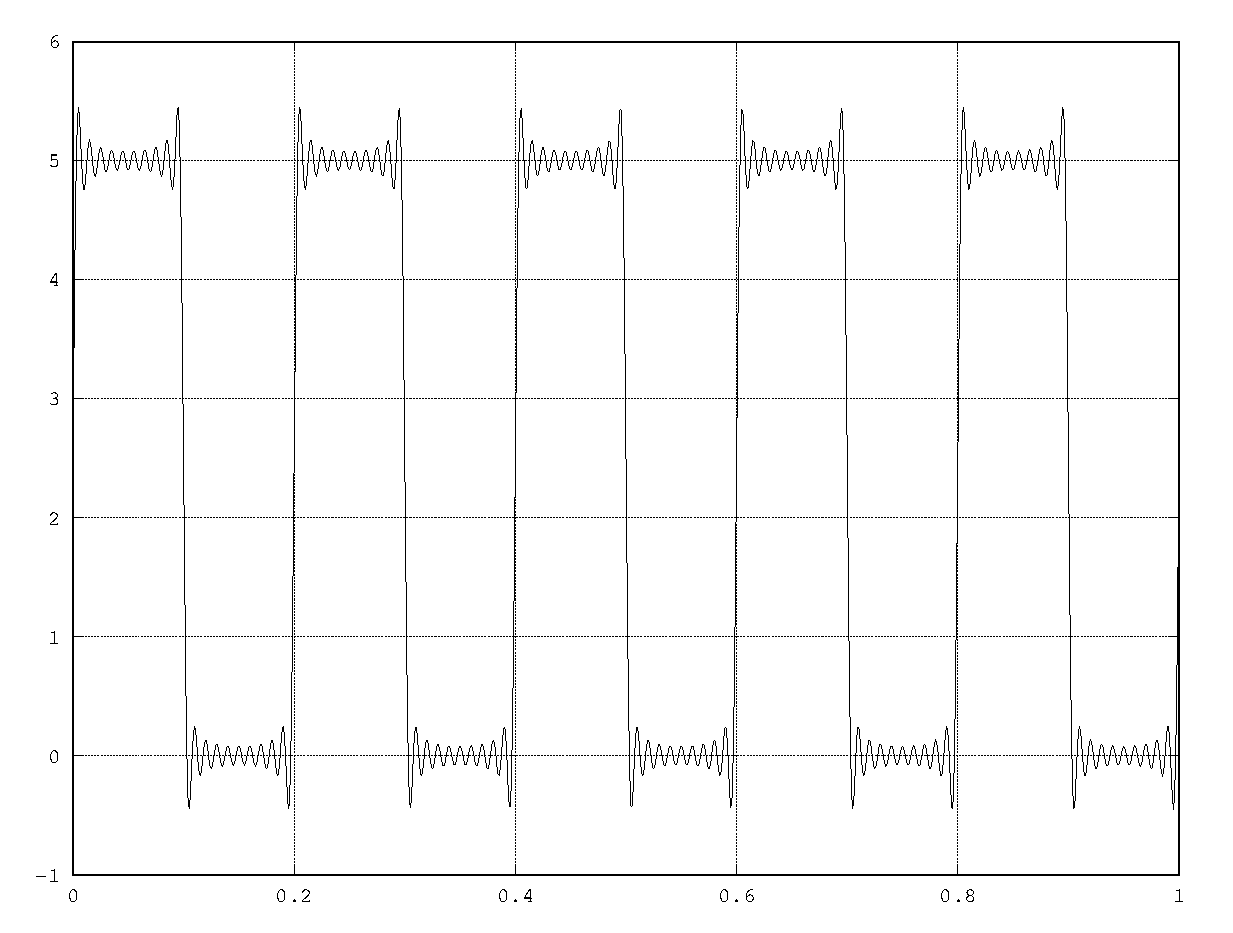
\includegraphics[width=\columnwidth]{chapter1/filter_input}
%%\vspace*{-13cm}
%\caption{Generating square wave using a fourier series.}
%\label{fig:clock}
%\end{figure}


%
\section{Filter}
%
%\chapter{The Optimum Receiver}

%\subsection{RC Circuit}
%
\begin{problem}
Refer to the circuit in Fig. \ref{fig:2.1}. Suppose you are told that $C$ has a resistance given by $\frac{1}{s  C}$.   Find the ratio $H(s)$ of the output voltage and input voltage using node analysis.  The above circuit is known as a low pass filter and $H(s)$ is known as the transfer function.
\end{problem}
%
%
\begin{figure}[!h]
\centering
\includegraphics[width=\columnwidth]{./figs/2.1.eps}
%\vspace*{-13cm}
\caption{Three stage $R-C$ low pass filter circuit}
\label{fig:2.1}
\end{figure}
%

\solution The equations at the nodes are given by
%
\begin{align}
\frac{V_1-V_i}{R}+ {sCV_1} + \frac{V_1-V_2}{R} &= 0
\\
\frac{V_2-V_1}{R}+ {sCV_2} + \frac{V_2-V_o}{R} &= 0
\\
\frac{V_o-V_2}{R}+ {sCV_o} &= 0
\end{align}
%
which can be expressed as
%
\begin{equation}
\begin{pmatrix}
sC + \frac{2}{R} & -\frac{1}{R} & 0 
\\
-\frac{1}{R}  & sC + \frac{2}{R} & -\frac{1}{R}
\\
0 & -\frac{1}{R} & sC + \frac{1}{R} 
\end{pmatrix}
\begin{pmatrix}
\frac{V_1}{V_i}
\\
\frac{V_2}{V_i}
\\
\frac{V_o}{V_i}
\end{pmatrix}
= 
\begin{pmatrix}
\frac{1}{R}
\\
0
\\
0
\end{pmatrix}
\end{equation}
%
Thus,
\begin{align}
H(s) &= \frac{V_o}{V_i} = 
\frac{
\begin{vmatrix}
sC + \frac{2}{R} & -\frac{1}{R} & \frac{1}{R}
\\
-\frac{1}{R}  & sC + \frac{2}{R} & 0
\\
0 & -\frac{1}{R} & 0
\end{vmatrix}
}{
\begin{vmatrix}
sC + \frac{2}{R} & -\frac{1}{R} & 0 
\\
-\frac{1}{R}  & sC + \frac{2}{R} & -\frac{1}{R}
\\
0 & -\frac{1}{R} & sC + \frac{1}{R} 
\end{vmatrix}
}
\\
&= \frac{1/R^3}{\brak{sC + \frac{1}{R} }\cbrak{\brak{sC + \frac{2}{R} }^2-\frac{1}{R^2}}-\frac{1}{R^2}\brak{sC + \frac{2}{R} }}
\end{align}
%
which can be expressed as
%
\begin{align}
H(s) &= \frac{1}{\brak{sCR + 1 }\cbrak{\brak{sCR + 2 }^2-1}-\brak{sCR + 2 }}
\\
&= \frac{1}{\brak{sCR + 2 }^3 - \brak{sCR + 2 }^2 - 2\brak{sCR + 2 } + 1}
\\
&= \frac{1}{\brak{sCR}^3 - 5 \brak{sCR }^2 + 6sCR  + 1}
\label{lpf_laplace}
\end{align}
%
\begin{problem}
Substitute $s = \jmath 2\pi f, \jmath =  \sqrt{-1}$ in \eqref{lpf_laplace} to obtain $H(f)$.  
$H(f)$ is 
known as the frequency response. Plot $\abs{H(f)}$ in octave for $-20 < f < 20$, given that $R = 1 \,k\Omega$ and $C = 10 \,\mu F$.
\end{problem}
%
\solution 
%
Type  the following code to get Fig. \ref{fig:filter_plot}.  You will find that $H(f)$ is a low pass
filter.
%
\begin{lstlisting}
wget https://raw.githubusercontent.com/gadepall/EE1310/master/fourier/series/codes/2.2.py
\end{lstlisting}

%\lstinputlisting[language=octave]{./codes/2.2.py}
%
\begin{figure}[!h]
\centering
\includegraphics[width=\columnwidth]{./figs/2.2.eps}
%\vspace*{-13cm}
\caption{Frequency response of the $R-C$ filter}
\label{fig:filter_plot}
\end{figure}
\begin{problem}
Find the frequency at which $\abs{H(f)}^2 = \frac{1}{2}$. This frequency is
known as the 3-dB bandwidth of $H(f)$.
\end{problem}
%
\solution Substituting $sCR = \jmath x$ in \eqref{lpf_laplace},
%
\begin{align}
 \abs{H(\jmath x)} &= \frac{1}{\sqrt{2}} \\
 \Rightarrow 
 -\jmath x^3 + 5x^2 +\jmath 6x + 1 &= \sqrt{2} \\
\Rightarrow 
 x^2(6-x^2)^2 + (1+5x^2)^2 &= 2 \\
 \Rightarrow 
x^6 + 13x^4 + 46x^2 -1&= 0 
\end{align}
%
Letting $y=x^2$, we obtain the cubic equation
%
\begin{align}
y^3 + 13y^2 + 46 y -1 = 0
\end{align}
%
The following script gives the 3 dB bandwidth for the filter H by choosing the 
real root.
%
\begin{lstlisting}
wget https://raw.githubusercontent.com/gadepall/EE1310/master/fourier/series/codes/2.3.py
\end{lstlisting}

%\lstinputlisting[language=python]{./codes/2.3.py}
%
This yields the value $f_{3\, dB} = 2.3395$ Hz.
\begin{problem}
Obtain the 3 dB bandwidth by solving the cubic equation in the previous problem
\end{problem}
%
\solution In the above, let $y = z - \frac{13}{3}$.  Then the equation becomes
%%
\begin{align}
\Rightarrow z^3 - (31/3)z  -1015/27  & = 0
\end{align}
%%
This equation has the theoretical solution evaluated by the following script
%
\begin{lstlisting}
wget https://raw.githubusercontent.com/gadepall/EE1310/master/fourier/series/codes/2.4.py
\end{lstlisting}

%\lstinputlisting[language=octave]{./codes/2.4.py}
Note that this script gives the same result as the one in the previous problem.
%Let
%%
%\begin{equation}
%\begin{split}
%q &= -31/3\\
%r &= -1135/9
%\end{split}
%%
%\end{equation}
%%
%Then
%%
%\begin{align}
%y = \cbrak{-\frac{r}{2} + \sqrt{\frac{r^2}{4} + \frac{q^3}{27}} }^{\frac{1}{3}} + \cbrak{-\frac{r}{2} - \sqrt{\frac{r^2}{4} + \frac{q^3}{27}} }^{\frac{1}{3}} - \frac{13}{3}
%\end{align}
%%
%and
%%
%\begin{align}
%x = \sbrak{\cbrak{-\frac{r}{2} + \sqrt{\frac{r^2}{4} + \frac{q^3}{27}} }^{\frac{1}{3}} + \cbrak{-\frac{r}{2} - \sqrt{\frac{r^2}{4} + \frac{q^3}{27}} }^{\frac{1}{3}} - \frac{13}{3}}^{\frac{1}{2}}
%\end{align}
%
\begin{problem}
\label{filter_op}
Suppose the square wave in Fig. \ref{fig:1.1} is given as input to the filter in Fig. \ref{fig:filter_plot}.  Find and plot the filter output.
\end{problem}
%
\solution  Using sinusoidal steady state analysis, if the input to the filter is
%
$\cos{2\pi n f t}$, the output is given by
\begin{equation}
\abs{H(nf)}\cos\cbrak{2\pi n f t + \angle H(nf)}
\end{equation}
%
Using the principle of superposition, for the input 
%
\begin{equation}
\sum_{n=0}^{\infty}a_n\cos 2\pi n f t + b_n \sin 2 \pi n f t
\end{equation}
%
the output will be
%
%
\begin{multline}
\sum_{n=0}^{\infty}a_n\abs{H(nf)}\cos\cbrak{2\pi n f t + \angle H(nf)} 
\\
+ b_n \abs{H(nf)}\sin\cbrak{2\pi n f t + \angle H(nf)}
\end{multline}
%
Suitably modifying the program in Problem \ref{fourier_series},
%
\begin{lstlisting}
wget https://raw.githubusercontent.com/gadepall/EE1310/master/fourier/series/codes/2.5.py
\end{lstlisting}
%\lstinputlisting[language=python]{./codes/2.5.py}
%
The output of the filter is shown  in Fig. \ref{fig:2.5}
\begin{figure}[!h]
\centering
\includegraphics[width=\columnwidth]{./figs/2.5.eps}
%\vspace*{-13cm}
\caption{Output of the $R-C$ filter}
\label{fig:2.5}
\end{figure}
%
\begin{problem}
Run the program in problem \ref{filter_op} by changing the for loop to
\begin{verbatim}
for n in range(2):
\end{verbatim}
Compare this output with the one in Fig. \ref{fig:2.5} by plotting in the same graph.
\end{problem}
\begin{problem}
Interpret the result in problem \ref{filter_op}.
\end{problem}
%
\solution
In Fig. \ref{fig:filter_plot}, $\abs{H(0)} = 1$ and $\abs{H(50)} = 0.02$.  All other values of $H$ are very small.  $\abs{H(0)} = 1$ contributes the DC component and $\abs{H(50)} = 0.02$ yields the sinusoidal component of 50 Hz.  Thus, $H(f)$ filters all higher harmonics in the square wave in Fig. \ref{fig:1.1}.
%\begin{problem}
%Sketch $\abs{H(nf)}$.
%\end{problem}
%%
%\solution
%\lstinputlisting[language=octave]{./codes/2.6.m}
%%
%The output of the filter is shown  in Fig. \ref{fig:2.6}
%\begin{figure}[!h]
%\centering
%\includegraphics[width=\columnwidth]{./figs/2.6.eps}
%%\vspace*{-13cm}
%\caption{Frequency response of the $R-C$ filter}
%\label{fig:2.6}
%\end{figure}
%%

%\begin{problem}
%Connect $g(t)$ to the following circuit for $R = 10 \,k \Omega, C = 10 \,\mu F$ and observe the output $v(t)$.  Measure the amplitude and time period of $v(t)$.
%\end{problem}
%\subsection{Circuit Analysis}
%%
%\begin{problem}
%	Obtain the expression for $H(s)$ using mesh analysis.
%\end{problem}
%%
%\begin{problem}
%	Repeat the above exercise using Thevenin's theorem.
%	\end{problem}
%	%
%	\begin{problem}
%		Repeat the above exercise using Norton's theorem.
%		\end{problem}
%	%
%	\begin{problem}
%		Repeat the above exercise using $Y-\Delta$ transformation.
%	\end{problem}
%\begin{problem}
%	Obtain all the two port network parameters for the circuit in Fig. \ref{fig:2.1}.
%\end{problem}
%			
%\begin{problem}
%For $R = 10 \,k \Omega, C = 1 \,\mu F$, plot $H(f)$ with respect to $f$.  Comment.
%\end{problem}
%\subsection{RL Circuit}
%%
%\begin{problem}
	%Using node analysis, design an $R-L$ circuit with the same frequency response as the $R-C$ circuit in the previous section.  Comment.
%\end{problem}
%%
%\begin{problem}
%Obtain the frequency response for this $R-L$ circuit using mesh analysis.
	%\end{problem}
	%%
%\begin{problem}
%Repeat the above exercise using Thevenin's theorem.
%\end{problem}
		%%
		%\begin{problem}
%Repeat the above exercise using Norton's theorem.
			%\end{problem}

%\subsection{Bandpass Filter}
%%
%\begin{problem}
	%Design an $R-C$ bandpass filter  and use it to filter a higher harmonic from the square wave generated using the arduino.
%\end{problem}
%%
%\begin{problem}
%Obtain the frequency response of the above filter.
%\end{problem}
%%
%\begin{problem}
%Obtain the above frequency response using an $RLC$ circuit.
%\end{problem}
%

%%\chapter{The Optimum Receiver}

\subsection{RC Circuit}
%
\begin{problem}
Refer to the circuit in Fig. \ref{fig:2.1}. Suppose you are told that $C$ has a resistance given by $\frac{1}{s  C}$.   Find the ratio $H(s)$ of the output voltage and input voltage using node analysis.  The above circuit is known as a low pass filter and $H(s)$ is known as the transfer function.
\end{problem}
%
%
\begin{figure}[!h]
\centering
\includegraphics[width=\columnwidth]{./chapter2/figs/2.1.eps}
%\vspace*{-13cm}
\caption{Three stage $R-C$ low pass filter circuit}
\label{fig:2.1}
\end{figure}
%

\solution The equations at the nodes are given by
%
\begin{align}
\frac{V_1-V_i}{R}+ {sCV_1} + \frac{V_1-V_2}{R} &= 0
\\
\frac{V_2-V_1}{R}+ {sCV_2} + \frac{V_2-V_o}{R} &= 0
\\
\frac{V_o-V_2}{R}+ {sCV_o} &= 0
\end{align}
%
which can be expressed as
%
\begin{equation}
\begin{pmatrix}
sC + \frac{2}{R} & -\frac{1}{R} & 0 
\\
-\frac{1}{R}  & sC + \frac{2}{R} & -\frac{1}{R}
\\
0 & -\frac{1}{R} & sC + \frac{1}{R} 
\end{pmatrix}
\begin{pmatrix}
\frac{V_1}{V_i}
\\
\frac{V_2}{V_i}
\\
\frac{V_o}{V_i}
\end{pmatrix}
= 
\begin{pmatrix}
\frac{1}{R}
\\
0
\\
0
\end{pmatrix}
\end{equation}
%
Thus,
\begin{align}
H(s) &= \frac{V_o}{V_i} = 
\frac{
\begin{vmatrix}
sC + \frac{2}{R} & -\frac{1}{R} & \frac{1}{R}
\\
-\frac{1}{R}  & sC + \frac{2}{R} & 0
\\
0 & -\frac{1}{R} & 0
\end{vmatrix}
}{
\begin{vmatrix}
sC + \frac{2}{R} & -\frac{1}{R} & 0 
\\
-\frac{1}{R}  & sC + \frac{2}{R} & -\frac{1}{R}
\\
0 & -\frac{1}{R} & sC + \frac{1}{R} 
\end{vmatrix}
}
\\
&= \frac{1/R^3}{\brak{sC + \frac{1}{R} }\cbrak{\brak{sC + \frac{2}{R} }^2-\frac{1}{R^2}}-\frac{1}{R^2}\brak{sC + \frac{2}{R} }}
\end{align}
%
which can be expressed as
%
\begin{align}
H(s) &= \frac{1}{\brak{sCR + 1 }\cbrak{\brak{sCR + 2 }^2-1}-\brak{sCR + 2 }}
\\
&= \frac{1}{\brak{sCR + 2 }^3 - \brak{sCR + 2 }^2 - 2\brak{sCR + 2 } + 1}
\\
&= \frac{1}{\brak{sCR}^3 - 5 \brak{sCR }^2 + 6sCR  + 1}
\label{lpf_laplace}
\end{align}
%
\begin{problem}
Substitute $s = \j 2\pi f, \j =  \sqrt{-1}$ in \eqref{lpf_laplace} to obtain $H(f)$.  $H(f)$ is known as the frequency response. Plot $\abs{H(f)}$ in octave for $-20 < f < 20$, given that $R = 1 \,k\Omega$ and $C = 10 \,\mu F$.
\end{problem}
%
\solution 
%
Type  the following code to get Fig. \ref{fig:filter_plot}.  You will find that $H(f)$ is a low pass
filter.
%
\lstinputlisting[language=octave]{./chapter2/codes/2.2.py}
%
\begin{figure}[!h]
\centering
\includegraphics[width=\columnwidth]{chapter2/figs/2.2.eps}
%\vspace*{-13cm}
\caption{Frequency response of the $R-C$ filter}
\label{fig:filter_plot}
\end{figure}
\begin{problem}
Find the frequency at which $\abs{H(f)}^2 = \frac{1}{2}$. This frequency is
known as the 3-dB bandwidth of $H(f)$.
\end{problem}
%
\solution Substituting sCR = \j x in \eqref{lpf_laplace},
%
\begin{align}
 \abs{H(\j x)} &= \frac{1}{\sqrt{2}} \\
 \Rightarrow 
 -jx^3 + 5x^2 +j6x + 1 &= \sqrt{2} \\
\Rightarrow 
 x^2(6-x^2)^2 + (1+5x^2)^2 &= 2 \\
 \Rightarrow 
x^6 + 13x^4 + 46x^2 -1&= 0 
\end{align}
%
Letting $y=x^2$, we obtain the cubic equation
%
\begin{align}
y^3 + 13y^2 + 46 y -1 = 0
\end{align}
%
The following script gives the 3 dB bandwidth for the filter H by choosing the 
real root.
%
\lstinputlisting[language=octave]{./chapter2/codes/2.3.py}
%
This yields the value $f_{3\, dB} = 2.3395$ Hz.
\begin{problem}
Obtain the 3 dB bandwidth by solving the cubic equation in the previous problem
\end{problem}
%
\solution In the above, let $y = z - \frac{13}{3}$.  Then the equation becomes
%%
\begin{align}
\Rightarrow z^3 - (31/3)z  -1015/27  & = 0
\end{align}
%%
This equation has the theoretical solution evaluated by the following script
%
\lstinputlisting[language=octave]{./chapter2/codes/2.4.py}
Note that this script gives the same result as the one in the previous problem.
%Let
%%
%\begin{equation}
%\begin{split}
%q &= -31/3\\
%r &= -1135/9
%\end{split}
%%
%\end{equation}
%%
%Then
%%
%\begin{align}
%y = \cbrak{-\frac{r}{2} + \sqrt{\frac{r^2}{4} + \frac{q^3}{27}} }^{\frac{1}{3}} + \cbrak{-\frac{r}{2} - \sqrt{\frac{r^2}{4} + \frac{q^3}{27}} }^{\frac{1}{3}} - \frac{13}{3}
%\end{align}
%%
%and
%%
%\begin{align}
%x = \sbrak{\cbrak{-\frac{r}{2} + \sqrt{\frac{r^2}{4} + \frac{q^3}{27}} }^{\frac{1}{3}} + \cbrak{-\frac{r}{2} - \sqrt{\frac{r^2}{4} + \frac{q^3}{27}} }^{\frac{1}{3}} - \frac{13}{3}}^{\frac{1}{2}}
%\end{align}
%
\begin{problem}
\label{filter_op}
Suppose the square wave in Fig. \ref{fig:1.1} is given as input to the filter in Fig. \ref{fig:filter_plot}.  Find and plot the filter output.
\end{problem}
%
\solution  Using sinusoidal steady state analysis, if the input to the filter is
%
$\cos{2\pi n f t}$, the output is given by
\begin{equation}
\abs{H(nf)}\cos\cbrak{2\pi n f t + \angle H(nf)}
\end{equation}
%
Using the principle of superposition, for the input 
%
\begin{equation}
\sum_{n=0}^{\infty}a_n\cos 2\pi n f t + b_n \sin 2 \pi n f t
\end{equation}
%
the output will be
%
%
\begin{multline}
\sum_{n=0}^{\infty}a_n\abs{H(nf)}\cos\cbrak{2\pi n f t + \angle H(nf)} 
\\
+ b_n \abs{H(nf)}\sin\cbrak{2\pi n f t + \angle H(nf)}
\end{multline}
%
Suitably modifying the program in Problem \ref{fourier_series},
%
\lstinputlisting[language=python]{./chapter2/codes/2.5.py}
%
The output of the filter is shown  in Fig. \ref{fig:2.5}
\begin{figure}[!h]
\centering
\includegraphics[width=\columnwidth]{./chapter2/figs/2.5.eps}
%\vspace*{-13cm}
\caption{Output of the $R-C$ filter}
\label{fig:2.5}
\end{figure}
%
\begin{problem}
Run the program in problem \ref{filter_op} by changing the for loop to
\begin{verbatim}
for n in range(2):
\end{verbatim}
Compare this output with the one in Fig. \ref{fig:2.5} by plotting in the same graph.
\end{problem}
\begin{problem}
Interpret the result in problem \ref{filter_op}.
\end{problem}
%
\solution
In Fig. \ref{fig:filter_plot}, $\abs{H(0)} = 1$ and $\abs{H(50)} = 0.02$.  All other values of $H$ are very small.  $\abs{H(0)} = 1$ contributes the DC component and $\abs{H(50)} = 0.02$ yields the sinusoidal component of 50 Hz.  Thus, $H(f)$ filters all higher harmonics in the square wave in Fig. \ref{fig:1.1}.
%\begin{problem}
%Sketch $\abs{H(nf)}$.
%\end{problem}
%%
%\solution
%\lstinputlisting[language=octave]{./chapter2/codes/2.6.m}
%%
%The output of the filter is shown  in Fig. \ref{fig:2.6}
%\begin{figure}[!h]
%\centering
%\includegraphics[width=\columnwidth]{./chapter2/figs/2.6.eps}
%%\vspace*{-13cm}
%\caption{Frequency response of the $R-C$ filter}
%\label{fig:2.6}
%\end{figure}
%%

%\begin{problem}
%Connect $g(t)$ to the following circuit for $R = 10 \,k \Omega, C = 10 \,\mu F$ and observe the output $v(t)$.  Measure the amplitude and time period of $v(t)$.
%\end{problem}
%\subsection{Circuit Analysis}
%%
%\begin{problem}
%	Obtain the expression for $H(s)$ using mesh analysis.
%\end{problem}
%%
%\begin{problem}
%	Repeat the above exercise using Thevenin's theorem.
%	\end{problem}
%	%
%	\begin{problem}
%		Repeat the above exercise using Norton's theorem.
%		\end{problem}
%	%
%	\begin{problem}
%		Repeat the above exercise using $Y-\Delta$ transformation.
%	\end{problem}
%\begin{problem}
%	Obtain all the two port network parameters for the circuit in Fig. \ref{fig:2.1}.
%\end{problem}
%			
%\begin{problem}
%For $R = 10 \,k \Omega, C = 1 \,\mu F$, plot $H(f)$ with respect to $f$.  Comment.
%\end{problem}
%\subsection{RL Circuit}
%%
%\begin{problem}
	%Using node analysis, design an $R-L$ circuit with the same frequency response as the $R-C$ circuit in the previous section.  Comment.
%\end{problem}
%%
%\begin{problem}
%Obtain the frequency response for this $R-L$ circuit using mesh analysis.
	%\end{problem}
	%%
%\begin{problem}
%Repeat the above exercise using Thevenin's theorem.
%\end{problem}
		%%
		%\begin{problem}
%Repeat the above exercise using Norton's theorem.
			%\end{problem}

%\subsection{Bandpass Filter}
%%
%\begin{problem}
	%Design an $R-C$ bandpass filter  and use it to filter a higher harmonic from the square wave generated using the arduino.
%\end{problem}
%%
%\begin{problem}
%Obtain the frequency response of the above filter.
%\end{problem}
%%
%\begin{problem}
%Obtain the above frequency response using an $RLC$ circuit.
%\end{problem}
%

%\input{./chapter2_code}
%	
%\newpage
%\section{Transients}
%%\chapter{The Optimum Receiver}

%\subsection{Transient Circuit}

\begin{problem}
Use an arduino to give a 5V input to the  circuit in Fig. \ref{fig:transient} with the switch closed.  Plot the output across the capacitor observed over 1 minute.  

	\begin{figure}[!h]
\centering
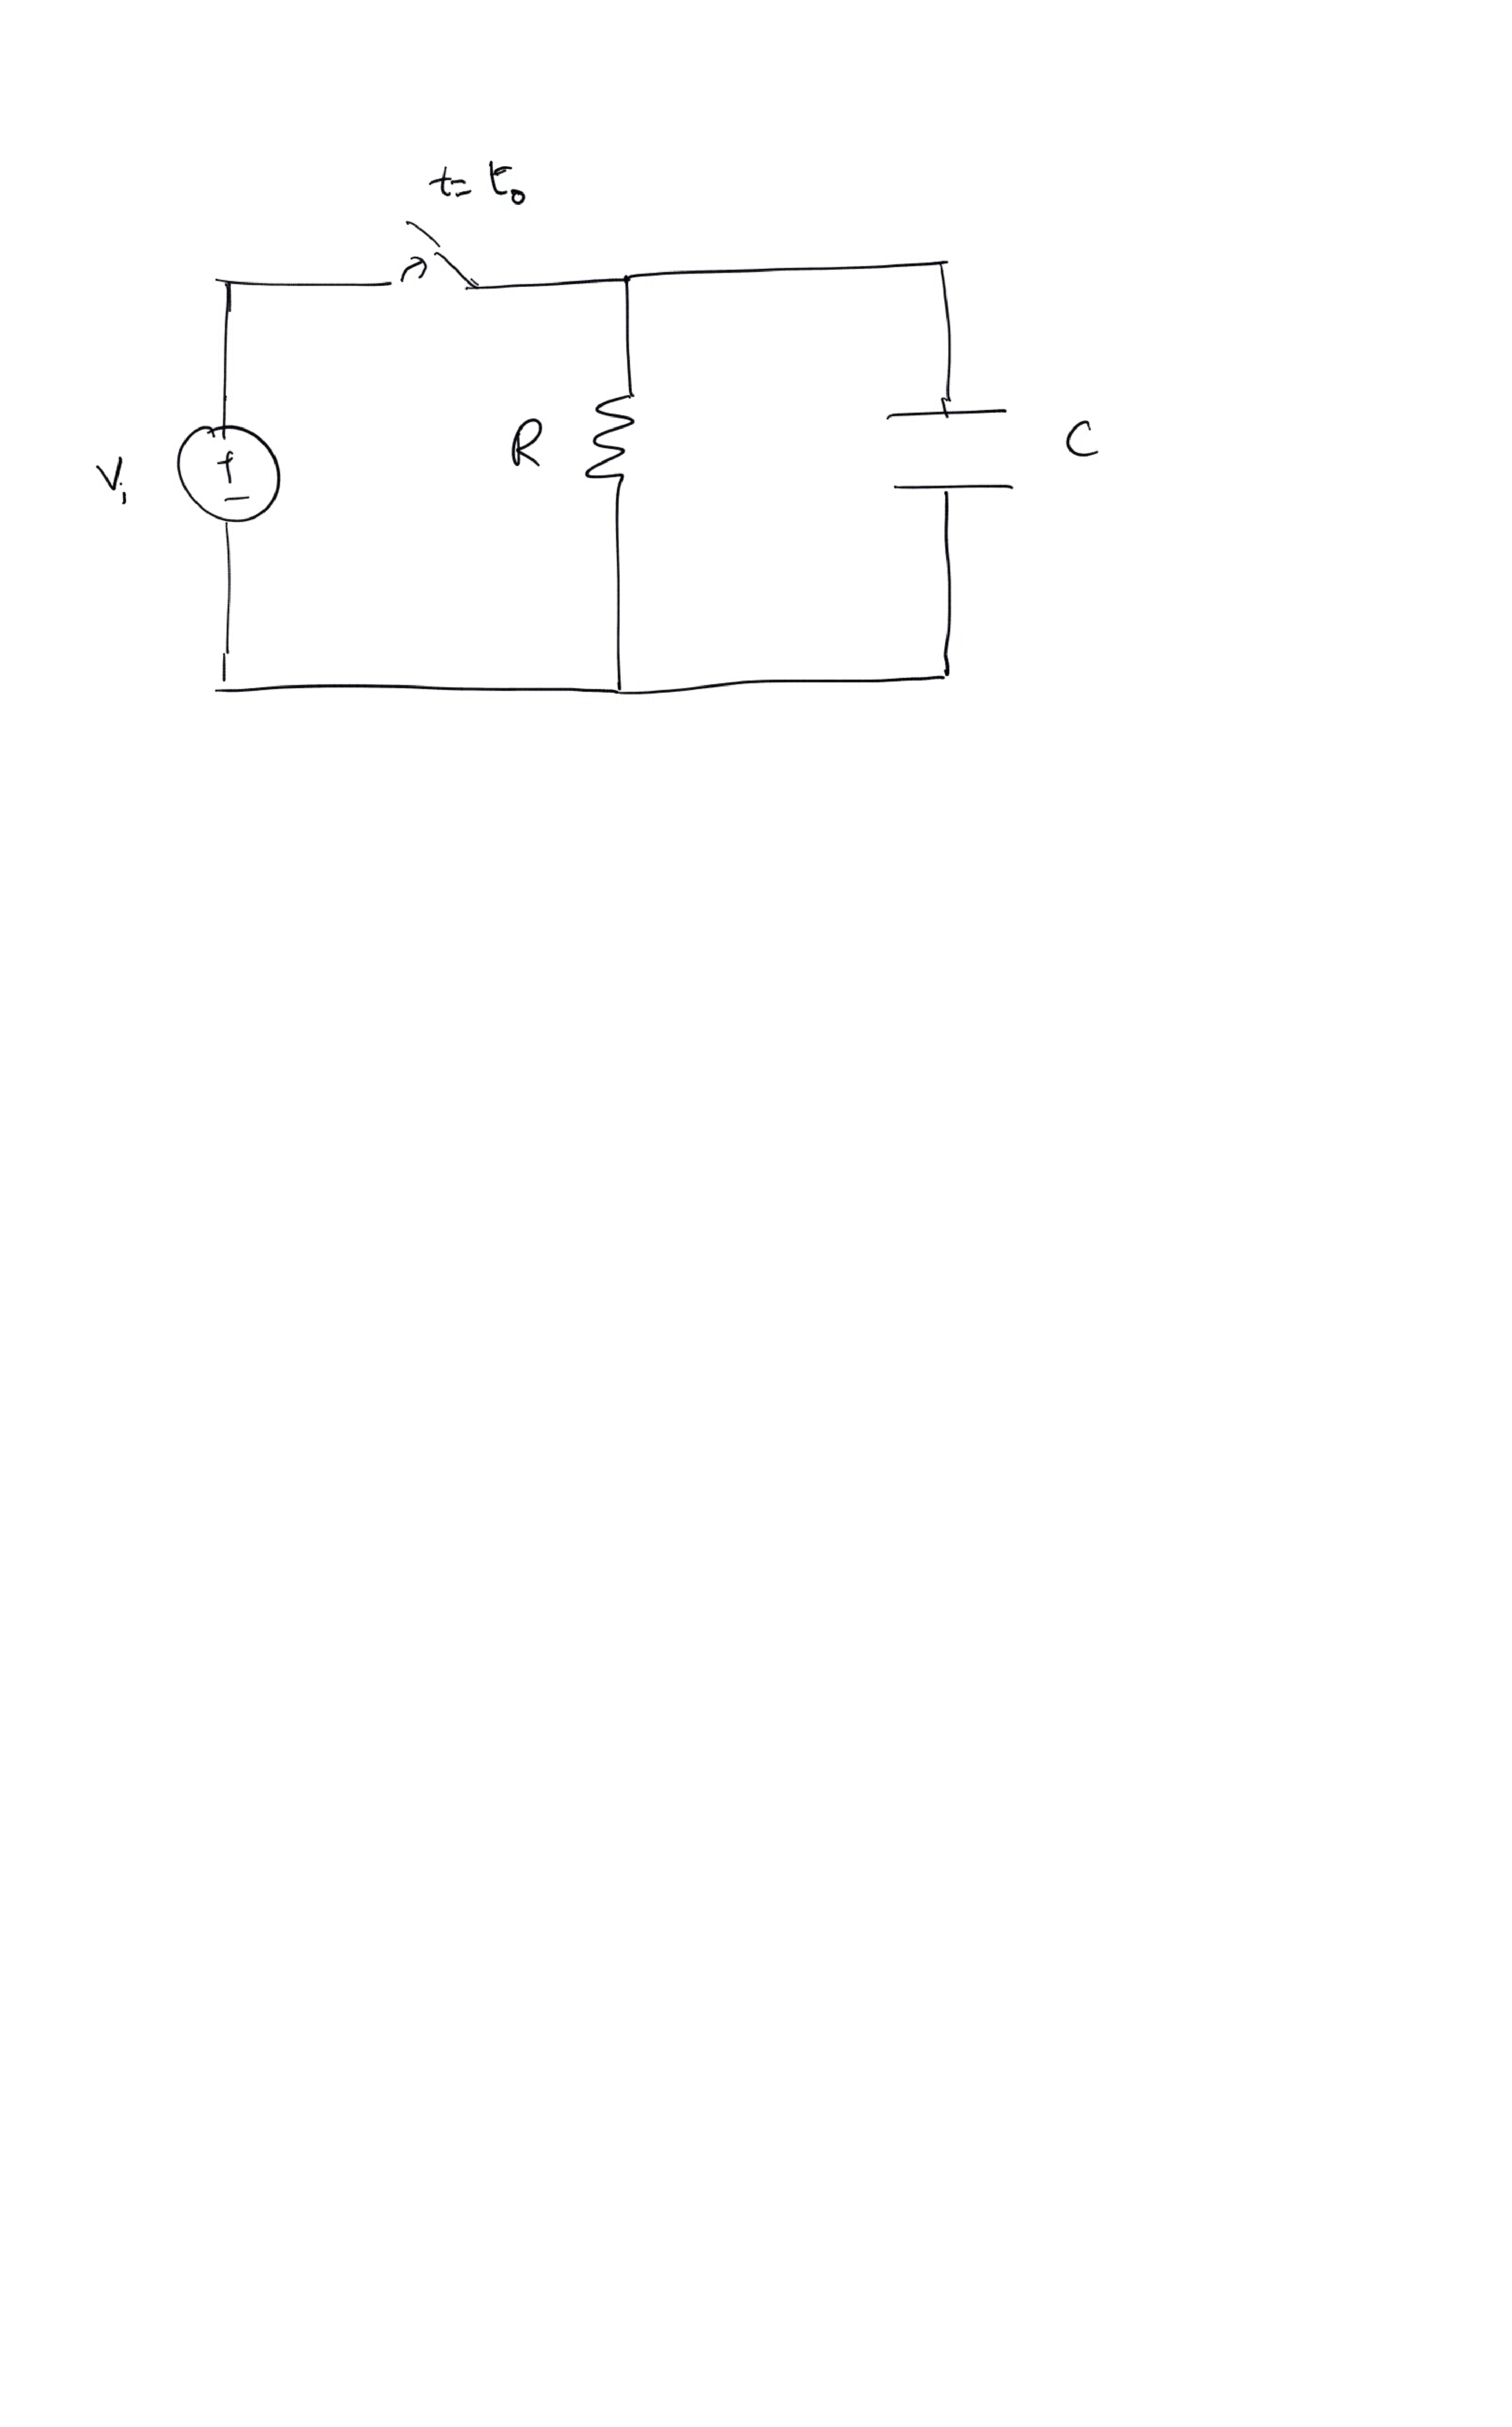
\includegraphics[width=\columnwidth]{chapter3/transient}
%\vspace*{-13cm}
\caption{$R-C$ filter for transient}
\label{fig:transient}
\end{figure}
\end{problem}
%
\begin{problem}
Open the switch and now plot the output observed across the capacitor over 1 minute.  
\end{problem}
%
\begin{problem}
Obtain the ouput using Laplace transforms for both cases.
\end{problem}
%
\begin{problem}
	Plot the theoretical and observed ouput.  Comment.
\end{problem}
\begin{problem}
	Find the impulse response of the $RC$ circuit
\end{problem}
\begin{problem}
	Using convolution, find the output.
\end{problem}

%
%\newpage
%\section{Application in Research}
%\input{revision}


%\bibliography{IEEEabrv,gvv_matrix}

%\input{chapter2} 
%%
%\newpage
%\section{$M$-ary Modulation}
%%\chapter{The Optimum Receiver}

%\subsection{Transient Circuit}

\begin{problem}
Use an arduino to give a 5V input to the  circuit in Fig. \ref{fig:transient} with the switch closed.  Plot the output across the capacitor observed over 1 minute.  

	\begin{figure}[!h]
\centering
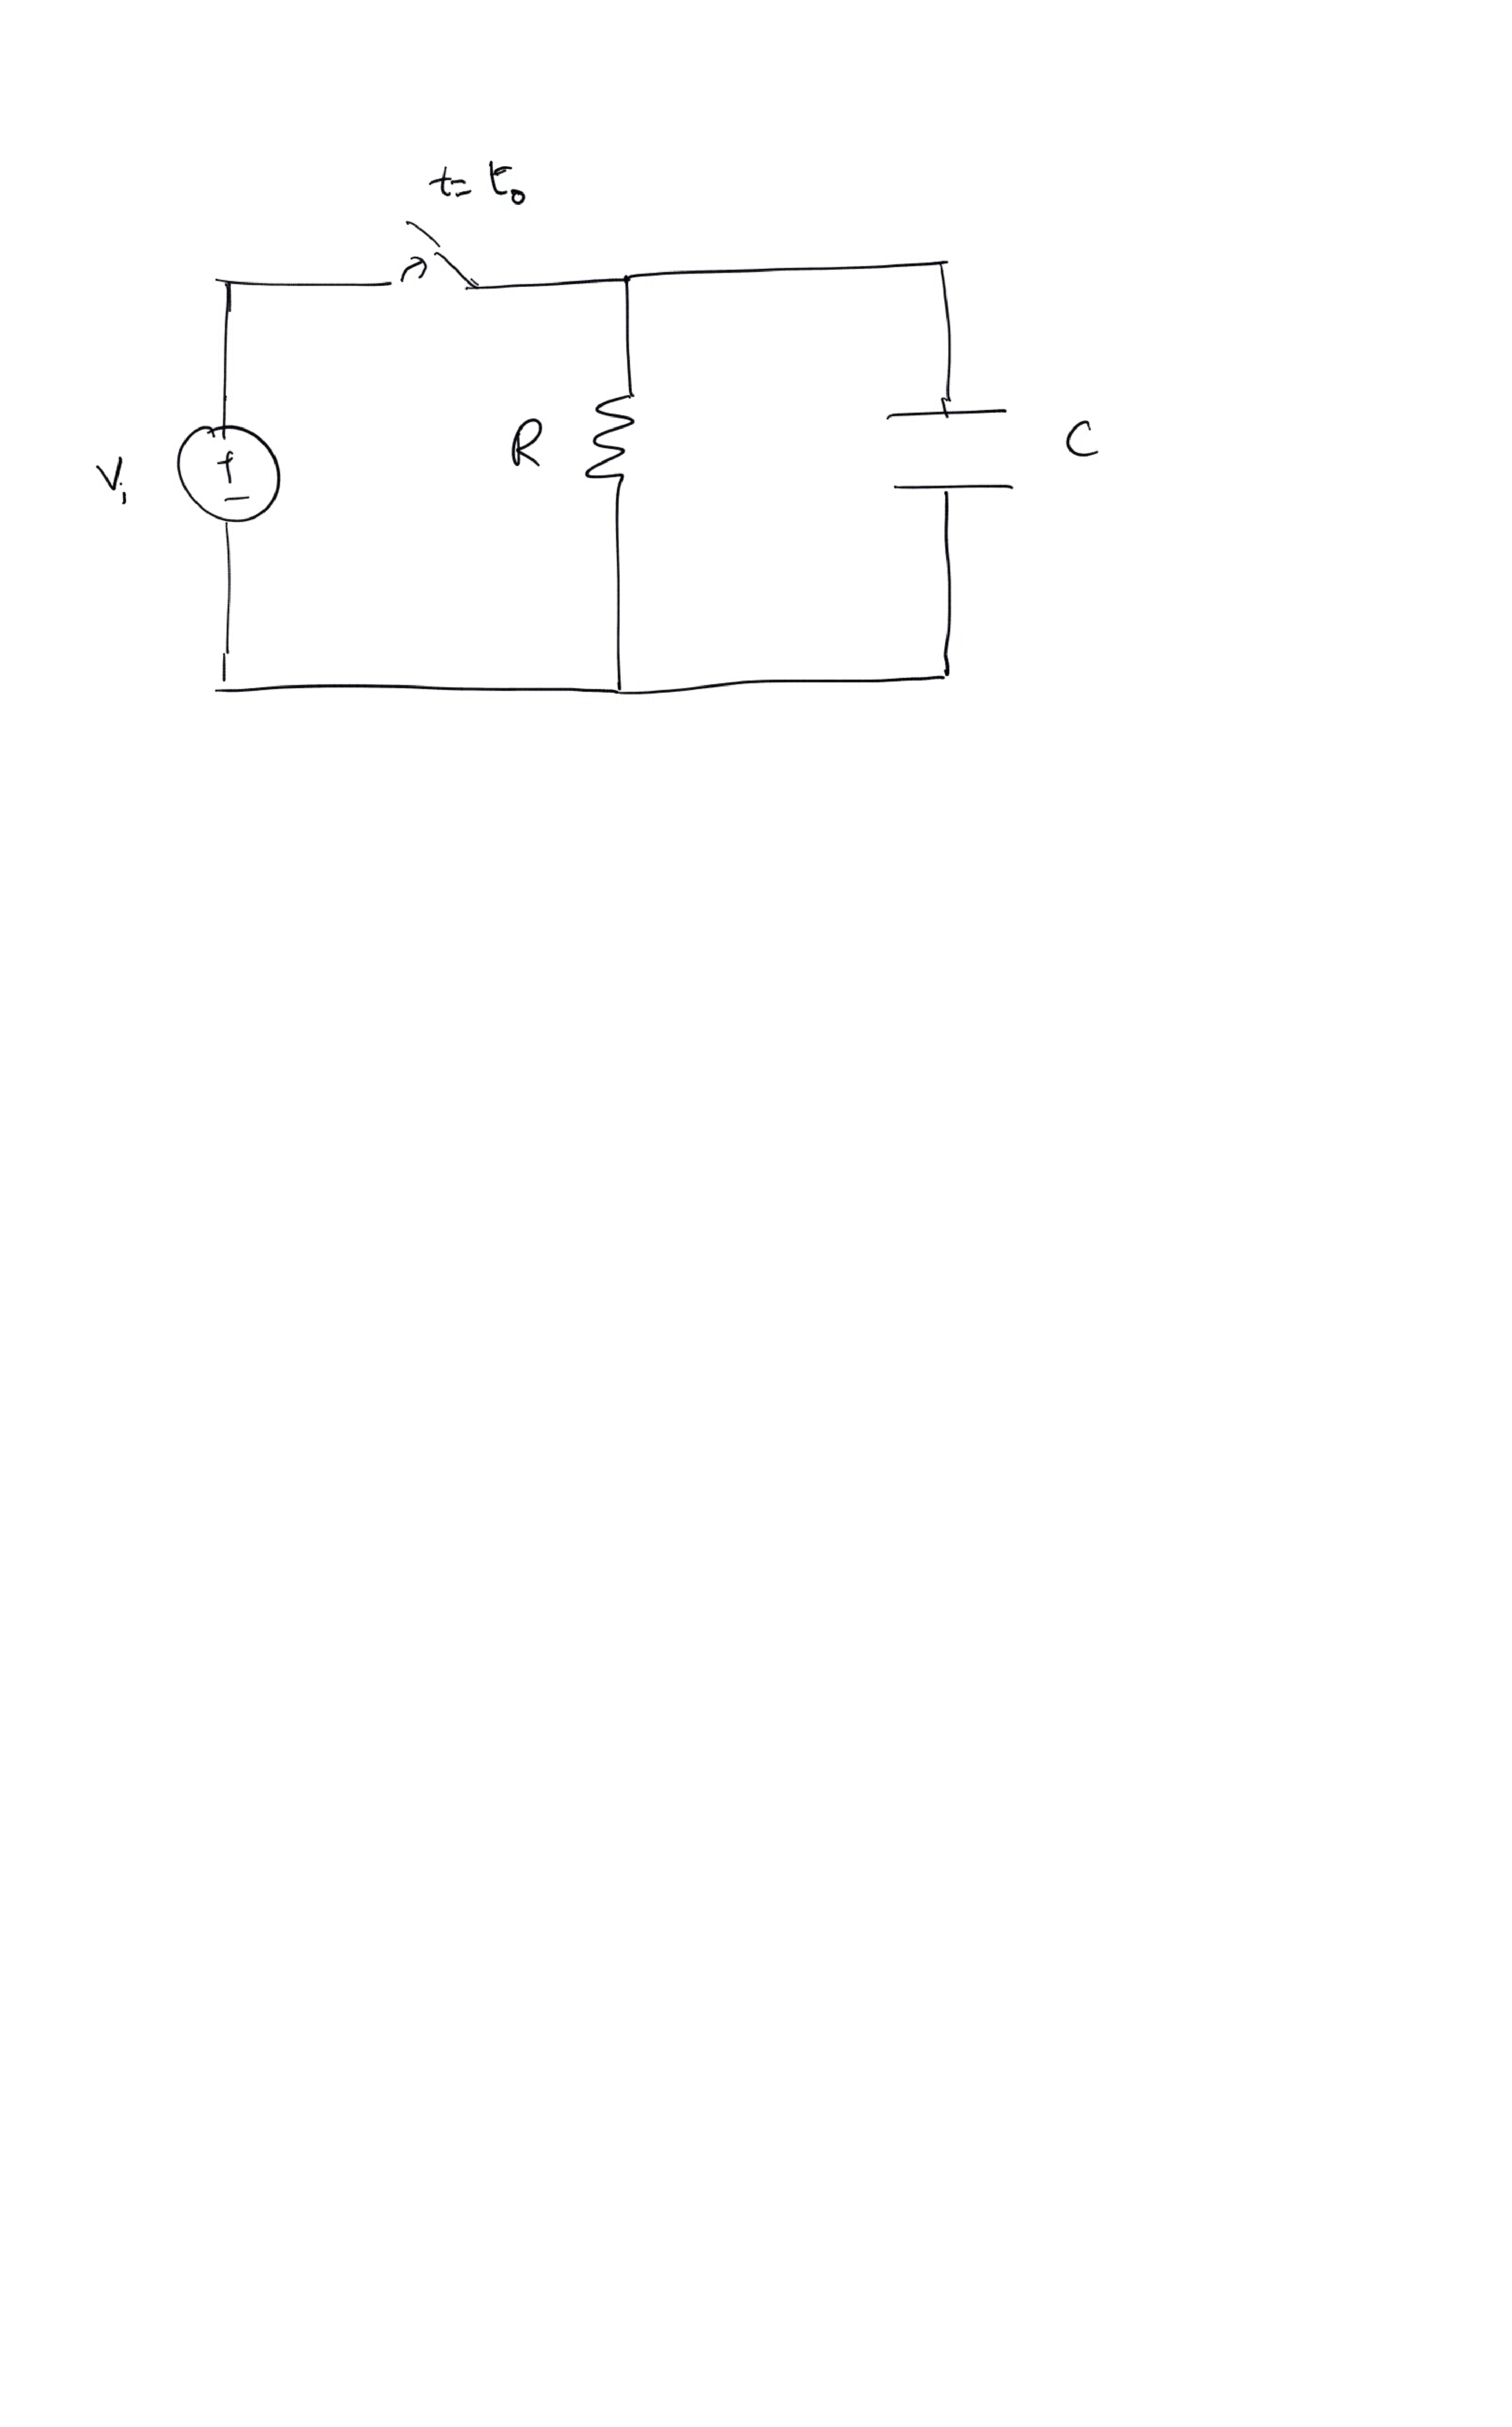
\includegraphics[width=\columnwidth]{chapter3/transient}
%\vspace*{-13cm}
\caption{$R-C$ filter for transient}
\label{fig:transient}
\end{figure}
\end{problem}
%
\begin{problem}
Open the switch and now plot the output observed across the capacitor over 1 minute.  
\end{problem}
%
\begin{problem}
Obtain the ouput using Laplace transforms for both cases.
\end{problem}
%
\begin{problem}
	Plot the theoretical and observed ouput.  Comment.
\end{problem}
\begin{problem}
	Find the impulse response of the $RC$ circuit
\end{problem}
\begin{problem}
	Using convolution, find the output.
\end{problem}
 
%
%\newpage
%\section{BER in Rayleigh Flat Slowly Fading Channels}
%\input{chapter4} 

\end{document}


